\documentclass{beamer}

\usepackage[slovene]{babel}
\usepackage{amsfonts,amssymb}
\usepackage[utf8]{inputenc}
\usepackage{lmodern}
\usepackage[T1]{fontenc}

\usetheme{Warsaw}

\newtheorem{izrek}{Izrek}
\newtheorem{definicija}{Definicija}
\newtheorem{primer}{Primer}
\newtheorem{trditev}{Trditev}
\newtheorem{oznaka}{Oznaka}

\newcommand{\pojem}[1]{\textsc{#1}}


\title{Fareyevo zaporedje in Riemannova hipoteza}
\author{Tjaša Vrhovnik}

\institute{Mentor: izr.~prof.~dr.~Aleš Vavpetič\\
	Univerza v Ljubljani\\
	Fakulteta za matematiko in fiziko\\
	Oddelek za matematiko}
\date{8.\ maj 2019}

\begin{document}

%%%%%%%%%%%%%%%%%%%%%%%%%%%%%%%%%%%%%%%%%%%

\begin{frame}
\titlepage
\end{frame}

%%%%%%%%%%%%%%%%%%%%%%%%%%%%%%%%%%%%%%%%%%%

\begin{frame}
\frametitle{Fareyevo zaporedje}

\pause
\begin{trditev}
Obstajajo $3003$ racionalna števila $\frac{p}{q}$, za katera velja $0<\frac{p}{q}<1$ ter je $q \leq 100$.
\end{trditev}

1751, R.~Flitcon

\end{frame}

%%%%%%%%%%%%%%%%%%%%%%%%%%%%%%%%%%%%%%%%%%%

\begin{frame}
\frametitle{Fareyevo zaporedje}

\begin{definicija}
\label{def:Farey}
\emph{Fareyevo zaporedje reda n} oz.\ \emph{n-to Fareyevo zaporedje} je množica racionalnih števil $\frac{p}{q}$ urejenih po velikosti, kjer sta $p$ in $q$ tuji si števili, ter velja $0 \leq p \leq q \leq n$. Označimo ga z $F_n$.

Ekvivalentno, $F_n$ vsebuje vse okrajšane ulomke med $0$ in $1$ z imenovalci, kvečjemu enakimi $n$.
\end{definicija}

\pause
\begin{definicija}
Sosednja člena v Fareyevem zaporedju imenujemo \emph{Fareyeva soseda}.
\end{definicija}

\end{frame}

%%%%%%%%%%%%%%%%%%%%%%%%%%%%%%%%%%%%%%%%%%%

\begin{frame}
\frametitle{Fareyevo zaporedje}

\begin{definicija}
Naj bosta $\frac{a}{b}$ in $\frac{c}{d}$ sosednja člena nekega Fareyevega zaporedja. Člen \[\frac{a+c}{b+d} \] imenujemo \emph{medianta}.
\end{definicija}

\pause
\begin{trditev}
Za medianto okrajšanih ulomkov \(\frac{a}{b} < \frac{c}{d}\) velja  \(\frac{a}{b} < \frac{a+c}{b+d} < \frac{c}{d}\) .
\end{trditev}

\pause
\begin{trditev}
Naj velja \( 0 \leq \frac{a}{b} < \frac{c}{d} \leq 1\). Ulomka $\frac{a}{b}$ in $\frac{c}{d}$ sta Fareyeva soseda v nekem Fareyevem zaporeju natanko tedaj, ko velja \(bc - ad = 1\).
\end{trditev}

\end{frame}

%%%%%%%%%%%%%%%%%%%%%%%%%%%%%%%%%%%%%%%%%%%

\begin{frame}
\frametitle{Fareyevo zaporedje}

\begin{definicija}
Preslikava \( \varphi \colon \mathbb{N} \rightarrow \mathbb{N}\), ki za vsako naravno število $n$ prešteje števila, manjša od $n$, ki so $n$ tuja, se imenuje \emph{Eulerjeva funkcija} $\varphi$.
\end{definicija}

\pause
\begin{trditev}
\label{trd:DolzinaZap}
Naj bo $\varphi$ Eulerjeva funkcija. Dolžina Fareyevega zaporedja reda n je
\[  |F_{n}| = |F_{n-1}| + \varphi(n). \]
\end{trditev}

\pause
\begin{trditev}
\label{trd:AsimptotDolzina}
Asimptotično se dolžina Fareyevega zaporedja obnaša kot
\[  |F_{n}|\sim\frac{3n^2}{\pi^2}. \]
\end{trditev}

\end{frame}

%%%%%%%%%%%%%%%%%%%%%%%%%%%%%%%%%%%%%%%%%%%%

\begin{frame}
\frametitle{Fordovi krogi}

\pause
\begin{definicija}
Naj bosta $p$ in $q$ tuji si števili v množici celih števil.
\emph{Fordov krog} C($\frac{p}{q}$) je krog v zgornji polravnini, ki se abscisne osi dotika v točki $\frac{p}{q}$, njegov polmer pa meri $\frac{1}{2q^2}$. 
\end{definicija}

\begin{center}
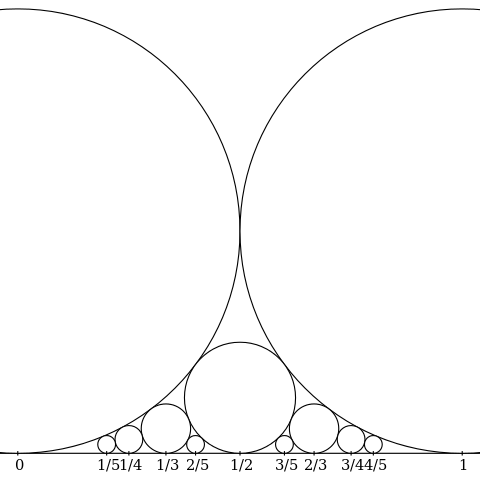
\includegraphics[scale=0.3]{fordov-krog.png}
\end{center}

\end{frame}

%%%%%%%%%%%%%%%%%%%%%%%%%%%%%%%%%%%%%%%%%%%%

\begin{frame}
\frametitle{Fordovi krogi}

\begin{trditev}
\label{trd:FordDisjTang}
Fordova kroga, ki pripadata različnima okrajšanima ulomkoma, sta bodisi tangentna bodisi disjunktna.
\end{trditev}

\pause
\begin{trditev}
\label{trd:FordTangentnost}
Fordova kroga C($\frac{a}{b}$) in C($\frac{c}{d}$) sta tangentna natanko tedaj, ko velja \( |bc-ad|=1. \)
\end{trditev}

\end{frame}

%%%%%%%%%%%%%%%%%%%%%%%%%%%%%%%%%%%%%%%%%%%%

\begin{frame}
\frametitle{Fordovi krogi}

\begin{definicija}
Tangentna Fordova kroga imenujemo \emph{Fordova soseda}.
\end{definicija}

\pause
\begin{izrek}
Naj bosta kroga C($\frac{p}{q}$) in C($\frac{P}{Q}$) Fordova soseda. Vse Fordove sosede Fordovega kroga C($\frac{p}{q}$) lahko zapišemo v obliki C($\frac{P_n}{Q_n}$), kjer je $\frac{P_n}{Q_n} = \frac{P+np}{Q+nq}$ in $n$ preteče vsa cela števila.
\end{izrek}

\end{frame}

%%%%%%%%%%%%%%%%%%%%%%%%%%%%%%%%%%%%%%%%%%%

\begin{frame}
\frametitle{Riemannova hipoteza}

\begin{itemize}
\pause
\item praštevila (Evklid, Euler)
%
\pause
\item $ \zeta(n) = \sum_{r=1}^{\infty}\frac{1}{r^n} $;  $n\in\mathbb{R}$
\end{itemize}

\pause
\begin{block}{Eulerjeva produktna formula}
\[ \sum_{n}\frac{1}{n^s} = \prod_{p}\frac{1}{1-p^{-s}}; n\in\mathbb{N}, p\in\mathbb{P} \]
\end{block}

Dokaz l.~1737, \emph{Variae observationes circa series infinitas}

\end{frame}

%%%%%%%%%%%%%%%%%%%%%%%%%%%%%%%%%%%%%%%%%%%

\begin{frame}
\frametitle{Riemannova hipoteza}

\begin{itemize}
\item Bernhard Riemann (1826 -- 1866)
\item l.~1859 razširi Eulerjevo definicijo
\end{itemize}

\begin{definicija}
\emph{Riemannova funkcija zeta} je za
 $s\in\mathbb{C}\backslash\{1\}$
definirana kot
\[ \zeta(s) = \sum_{n=1}^{\infty}\frac{1}{n^s}. \]
\end{definicija}

\end{frame}

%%%%%%%%%%%%%%%%%%%%%%%%%%%%%%%%%%%%%%%%%%%

\begin{frame}
\frametitle{Riemannova hipoteza}

\begin{block}{Riemannova hipoteza}
Vse netrivialne ničle Riemannove funkcije zeta ležijo na premici $s=\frac{1}{2}+it$.
\end{block}

\begin{center}
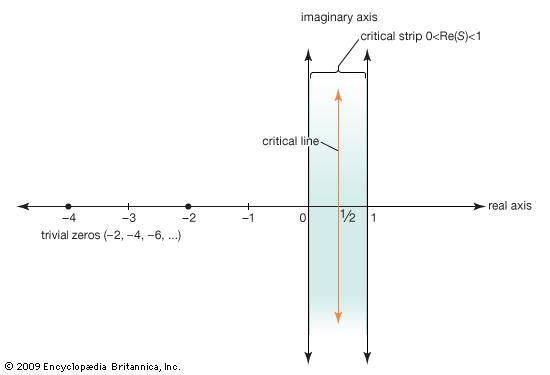
\includegraphics[scale=0.3]{zeta-funkcija.png}
\end{center}

\end{frame}

%%%%%%%%%%%%%%%%%%%%%%%%%%%%%%%%%%%%%%%%%%%

\begin{frame}
\frametitle{Riemannova hipoteza}

\begin{definicija}
Naj bo $k\in\mathbb{N}$. \emph{M\"obiusova funkcija} je definirana kot
\[
\mu(k) = \left\{
\begin{array}{rl}
0 & ;\ \mbox{k vsebuje kvadrat praštevila}\\
(-1)^p & ;\  \mbox{k je produkt p različnih praštevil.}
\end{array}
\right.
\]
\end{definicija}

\pause
\begin{definicija}
Za $n\in\mathbb{N}$ je \emph{Mertensova funkcija} definirana kot
\[ M(n)=\sum_{k\leq n}\mu(k).\]
\end{definicija}

\pause
\[ \forall\epsilon>0.\ M(n) = o(n^{1/2+\epsilon}) \iff \textrm{Riemannova hipoteza} \]

\end{frame}

%%%%%%%%%%%%%%%%%%%%%%%%%%%%%%%%%%%%%%%%%%%

\begin{frame}
\frametitle{Riemannova hipoteza}

\begin{definicija}
Naj bosta $L(n)$ dolžina Fareyevega zaporedja $F_{n}$ in $r_{v}$ njegov v-ti element. Definiramo razliko
\[ \delta_{v}= r_{v}-v/L(n). \]
\end{definicija}

\pause
Franel-Landau (1924):
\[ \forall\epsilon>0.\ \sum_{v=1}^{L(n)}|\delta_{v}| = o(n^{1/2+\varepsilon}) \iff \textrm{Riemannova hipoteza} \]

\end{frame}

%%%%%%%%%%%%%%%%%%%%%%%%%%%%%%%%%%%%%%%%%%%

\begin{frame}
\frametitle{Riemannova hipoteza}

Za vsak $\varepsilon > 0$ 
\[ \sum_{v=1}^{L(n)}|\delta_{v}| = o(n^{1/2+\varepsilon}) \iff M(n) = o(n^{1/2+\varepsilon}). \]

\end{frame}

%%%%%%%%%%%%%%%%%%%%%%%%%%%%%%%%%%%%%%%%%%%

\end{document}